%%Copyright 2021. Any replication of this document is permissible. The primary package of this document is from cjquines%%

%%PRIMARY PREAMBLE%%
\documentclass[12pt,paper=letter]{scrartcl}
\usepackage[ boxthm, parskip]{cjquines}
\usepackage{CJKutf8}


%%ADDITIONAL PACKAGES%%

\tikzset{every picture/.style={line width=0.75pt}} %set default line width to 0.75pt 
\newcommand{\ans}[1]{{\sffamily \bfseries Answer.}\;\(\boxed{\text{#1}}\).}
\newcommand{\ansb}[2]{{\sffamily \bfseries Answer.}\;\(\boxed{\text{(#1) #2}}\).}
\newcommand{\sol}{{\sffamily \bfseries Solution.}\;}
\newcommand{\soln}[1]{{\sffamily \bfseries Solution #1.}\;}
\newcommand{\back}[1]{{\sffamily \bfseries Background.}\;}
\newenvironment{rem}%
{\noindent \ignorespaces \small \sffamily \sansmath {\bfseries Remark.}}%
{\ignorespacesafterend}

\newcommand{\joshbluebf}[1]{{\bfseries \sffamily \color{DarkMidnightBlue} #1}}
\newcommand{\joshbf}[1]{{\bfseries \sffamily \color{black} #1}}



%%FONT FAMILY%%
%\renewcommand{\familydefault}{\sfdefault}%


\begin{document}


\title{Week 7 Some Olympiad Problems (Part I)}
\author{\joshbluebf{Problems of the Week — Season 2}}
\date{February 09, 2022}

\maketitle
\setlength{\unitlength}{1in}
\begin{picture}(2,0)
  \put(1.20,1.45){\hbox{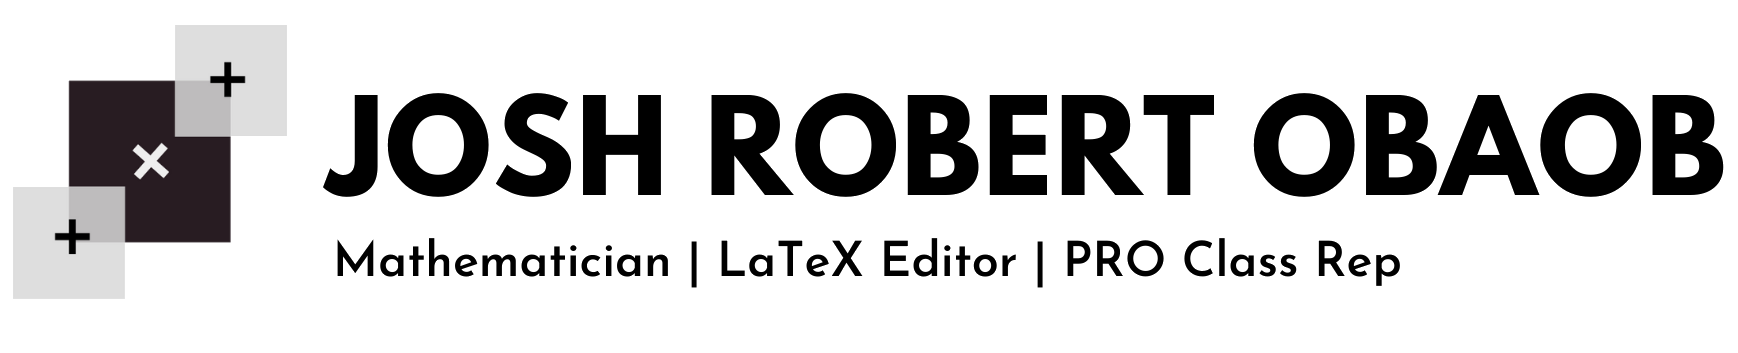
\includegraphics[width=4.2in]{logo2.png}}}
\end{picture}
\vspace{-2em}


\begin{abstract}
Hi! This is the \joshbf{seventh episode/article} of my mathematical series. In this article, this contains some random problems that I answered in preparation for the incoming \joshbf{24th Philippine Mathematical Olympiad (PMO) Qualifying Stage} this next week!. For this article, this is the \joshbf{PART 1} of \joshbf{Week 7}. I want to thank \joshbf{Sir Samuel Gayangos} of \joshbf{Zamboanga Chong Hua High School} for giving me some of the questions being compiled in the article. Before reading the solutions, try to solve these! Enjoy!
\end{abstract}

\vspace{-2em}

\section*{Problems}

\begin{problem}
Determine the maximum value of the difference of two positive integers whose sum is 2034 and whose product is a multiple of 2034.
\end{problem}

\begin{problem}
The area of the equilateral triangle $ABC$ is $8 + 4\sqrt{3}$ cm$^2$. $M$ is the midpoint of $BC$. The bisector of $\angle MAB$ intersects $BM$ at a point $N.$ What is the area, in cm$^2$, of triangle $ABN$?

\begin{center}
    


\tikzset{every picture/.style={line width=0.75pt}} %set default line width to 0.75pt        

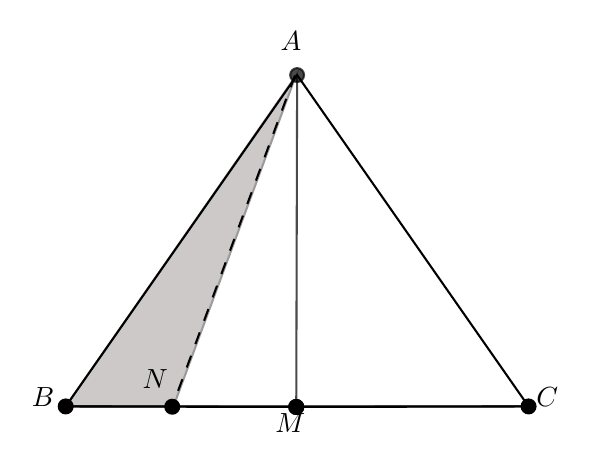
\begin{tikzpicture}[x=0.75pt,y=0.75pt,yscale=-1,xscale=1]
%uncomment if require: \path (0,499); %set diagram left start at 0, and has height of 499

%Shape: Right Triangle [id:dp45685224766566246] 
\draw  [color={rgb, 255:red, 155; green, 155; blue, 155 }  ,draw opacity=1 ][fill={rgb, 255:red, 129; green, 120; blue, 121 }  ,fill opacity=0.4 ] (334.97,102.15) -- (224.21,261.2) -- (276.13,261.2) -- cycle ;
%Straight Lines [id:da8013422245362609] 
\draw    (224.21,261.2) -- (335.29,261.46) ;
\draw [shift={(335.29,261.46)}, rotate = 0.13] [color={rgb, 255:red, 0; green, 0; blue, 0 }  ][fill={rgb, 255:red, 0; green, 0; blue, 0 }  ][line width=0.75]      (0, 0) circle [x radius= 3.35, y radius= 3.35]   ;
\draw [shift={(224.21,261.2)}, rotate = 0.13] [color={rgb, 255:red, 0; green, 0; blue, 0 }  ][fill={rgb, 255:red, 0; green, 0; blue, 0 }  ][line width=0.75]      (0, 0) circle [x radius= 3.35, y radius= 3.35]   ;
%Shape: Triangle [id:dp5043503310548794] 
\draw   (335.71,101.54) -- (447.22,261.2) -- (224.21,261.2) -- cycle ;
%Straight Lines [id:da9098078779949543] 
\draw    (447.22,261.2) -- (335.29,261.46) ;
\draw [shift={(335.29,261.46)}, rotate = 179.87] [color={rgb, 255:red, 0; green, 0; blue, 0 }  ][fill={rgb, 255:red, 0; green, 0; blue, 0 }  ][line width=0.75]      (0, 0) circle [x radius= 3.35, y radius= 3.35]   ;
\draw [shift={(447.22,261.2)}, rotate = 179.87] [color={rgb, 255:red, 0; green, 0; blue, 0 }  ][fill={rgb, 255:red, 0; green, 0; blue, 0 }  ][line width=0.75]      (0, 0) circle [x radius= 3.35, y radius= 3.35]   ;
%Straight Lines [id:da6144378132881774] 
\draw [color={rgb, 255:red, 0; green, 0; blue, 0 }  ,draw opacity=1 ] [dash pattern={on 4.5pt off 4.5pt}]  (334.63,101.76) -- (275.53,261.34) ;
\draw [shift={(275.53,261.34)}, rotate = 110.32] [color={rgb, 255:red, 0; green, 0; blue, 0 }  ,draw opacity=1 ][fill={rgb, 255:red, 0; green, 0; blue, 0 }  ,fill opacity=1 ][line width=0.75]      (0, 0) circle [x radius= 3.35, y radius= 3.35]   ;
%Straight Lines [id:da48882174888005814] 
\draw [color={rgb, 255:red, 0; green, 0; blue, 0 }  ,draw opacity=0.71 ]   (335.71,101.54) -- (335.29,261.46) ;
\draw [shift={(335.29,261.46)}, rotate = 90.15] [color={rgb, 255:red, 0; green, 0; blue, 0 }  ,draw opacity=0.71 ][fill={rgb, 255:red, 0; green, 0; blue, 0 }  ,fill opacity=0.71 ][line width=0.75]      (0, 0) circle [x radius= 3.35, y radius= 3.35]   ;
\draw [shift={(335.71,101.54)}, rotate = 90.15] [color={rgb, 255:red, 0; green, 0; blue, 0 }  ,draw opacity=0.71 ][fill={rgb, 255:red, 0; green, 0; blue, 0 }  ,fill opacity=0.71 ][line width=0.75]      (0, 0) circle [x radius= 3.35, y radius= 3.35]   ;


% Text Node
\draw (259.81,241.92) node [anchor=north west][inner sep=0.75pt]    {$N$};
% Text Node
\draw (323.74,263.21) node [anchor=north west][inner sep=0.75pt]    {$M$};
% Text Node
\draw (449.54,250.61) node [anchor=north west][inner sep=0.75pt]    {$C$};
% Text Node
\draw (206.39,250.47) node [anchor=north west][inner sep=0.75pt]    {$B$};
% Text Node
\draw (326.27,79.22) node [anchor=north west][inner sep=0.75pt]    {$A$};


\end{tikzpicture}
\end{center}
\end{problem}

\begin{problem}[\href{http://pmo.ph/wp-content/uploads/2014/08/19th-PMO-Qualifying-Stage-Questions-and-Answers.pdf}{PMO 19 Qualifying II.4}] If $b>1$, find the minimum value of $\dfrac{9b^2 -18b +`13}{b-1}$.

\end{problem}


\begin{problem}[\href{https://pmo.ph/wp-content/uploads/2019/01/21st-PMO-Qualifying-Stage.pdf}{PMO 21 Qualifying I.8}]
A bowl of negligible thickness is in the shape of a truncated circular cone, with height 4 in and upper and lower radii of 6 in and 9 in, respectively. What is the volume of the bowl?

\end{problem}

\begin{problem}[\href{http://pmo.ph/wp-content/uploads/2020/11/19th-PMO-Area-Stage-Questions-and-Answers.pdf}{PMO 19 Areas I.5}] In parallelogram $ABCD$, $AB=1, BC =4,$ and $\angle ABC = 60^{\circ}$. Suppose that $AC$ is extended from $A$ to a point $E$ beyond $C$ so that triangle $ADE$ has the same area as the parallelogram. Find the length of $DE.$

\end{problem}

\begin{problem}[\href{https://pmo.ph/wp-content/uploads/2019/01/21st-PMO-Area-Stage.pdf}{PMO 21 Areas I.20}]
Suppose that $a, b, c$ are real numbers such that

$$\dfrac{1}{a} + \dfrac{1}{b} + \dfrac{1}{c} = 4\left( \dfrac{1}{a+b} + \dfrac{1}{b+c} + \dfrac{1}{c+a} \right) = \dfrac{c}{a+b} + \dfrac{a}{b+c} + \dfrac{b}{c+a} = 4$$.

Determine the value of $abc.$

\begin{problem}[\href{https://www.facebook.com/cediesmathverse/posts/478611540322117}{Cedie's Mathverse Problem 3B}]

Find, with proof, all nonnegative integer triples $(x,y,z)$ such that $3^x = 7^y + 2^z$.
\end{problem}

\end{problem}

\vspace{15cm}

\begin{center}
    {\Large \textit{This is intentionally blank.}}
\end{center}


\newpage

\section*{Solutions}

\vspace{1cm}

\begin{probboxed}
Determine the maximum value of the difference of two positive integers whose sum is 2034 and whose product is a multiple of 2034.
\end{probboxed}

\ans{678}

\sol

Let $a$ and $b$ be the positive integers such that $a+b=2034$ and $ab = 2034k$ for some $k \in \mathbb{N}$. Recall that $(a-b)^2 = (a+b)^2 - 4ab$. But we are looking for the maximum of $a-b$. To make things easier, we will first find the maximum value of $k$ so that we can obtain the maximum value of $a-b$. We will do this in the following fashion:

\begin{equation*}
    \begin{array}{lll}
         (a+b)^2 - 4ab & \geq & 0 \\
         (2034)^2 -4(2034k) & \geq & 0 \\
         \\
        \qquad \qquad \qquad \qquad 4k & \leq & 2034 \\
        
        \\
        
        
        \qquad \qquad \qquad \qquad k & \leq & \dfrac{1017}{2} 
    \end{array}
\end{equation*}

Notice that $k$ is a non-integer. In order to obtain the maximum integer value of $k$, we check the integers below the non-integer value of $k$ that can satisfy the condition. Since $$(a-b) = 6\sqrt{(113)(1017-2k)}$$ and 113 is a prime number, this implies $k =452$ and it satisfies the condition!

\vspace{2mm}

Hence, \fbox{$(a-b) = 678$.}

\newpage

\begin{probboxed}
The area of the equilateral triangle $ABC$ is $8 + 4\sqrt{3}$ cm$^2$. $M$ is the midpoint of $BC$. The bisector of $\angle MAB$ intersects $BM$ at a point $N.$ What is the area, in cm$^2$, of triangle $ABN$?

\begin{center}
    


\tikzset{every picture/.style={line width=0.75pt}} %set default line width to 0.75pt        

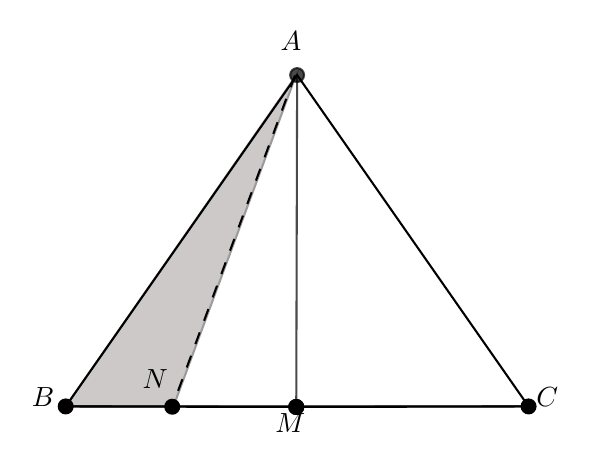
\begin{tikzpicture}[x=0.75pt,y=0.75pt,yscale=-1,xscale=1]
%uncomment if require: \path (0,499); %set diagram left start at 0, and has height of 499

%Shape: Right Triangle [id:dp45685224766566246] 
\draw  [color={rgb, 255:red, 155; green, 155; blue, 155 }  ,draw opacity=1 ][fill={rgb, 255:red, 129; green, 120; blue, 121 }  ,fill opacity=0.4 ] (334.97,102.15) -- (224.21,261.2) -- (276.13,261.2) -- cycle ;
%Straight Lines [id:da8013422245362609] 
\draw    (224.21,261.2) -- (335.29,261.46) ;
\draw [shift={(335.29,261.46)}, rotate = 0.13] [color={rgb, 255:red, 0; green, 0; blue, 0 }  ][fill={rgb, 255:red, 0; green, 0; blue, 0 }  ][line width=0.75]      (0, 0) circle [x radius= 3.35, y radius= 3.35]   ;
\draw [shift={(224.21,261.2)}, rotate = 0.13] [color={rgb, 255:red, 0; green, 0; blue, 0 }  ][fill={rgb, 255:red, 0; green, 0; blue, 0 }  ][line width=0.75]      (0, 0) circle [x radius= 3.35, y radius= 3.35]   ;
%Shape: Triangle [id:dp5043503310548794] 
\draw   (335.71,101.54) -- (447.22,261.2) -- (224.21,261.2) -- cycle ;
%Straight Lines [id:da9098078779949543] 
\draw    (447.22,261.2) -- (335.29,261.46) ;
\draw [shift={(335.29,261.46)}, rotate = 179.87] [color={rgb, 255:red, 0; green, 0; blue, 0 }  ][fill={rgb, 255:red, 0; green, 0; blue, 0 }  ][line width=0.75]      (0, 0) circle [x radius= 3.35, y radius= 3.35]   ;
\draw [shift={(447.22,261.2)}, rotate = 179.87] [color={rgb, 255:red, 0; green, 0; blue, 0 }  ][fill={rgb, 255:red, 0; green, 0; blue, 0 }  ][line width=0.75]      (0, 0) circle [x radius= 3.35, y radius= 3.35]   ;
%Straight Lines [id:da6144378132881774] 
\draw [color={rgb, 255:red, 0; green, 0; blue, 0 }  ,draw opacity=1 ] [dash pattern={on 4.5pt off 4.5pt}]  (334.63,101.76) -- (275.53,261.34) ;
\draw [shift={(275.53,261.34)}, rotate = 110.32] [color={rgb, 255:red, 0; green, 0; blue, 0 }  ,draw opacity=1 ][fill={rgb, 255:red, 0; green, 0; blue, 0 }  ,fill opacity=1 ][line width=0.75]      (0, 0) circle [x radius= 3.35, y radius= 3.35]   ;
%Straight Lines [id:da48882174888005814] 
\draw [color={rgb, 255:red, 0; green, 0; blue, 0 }  ,draw opacity=0.71 ]   (335.71,101.54) -- (335.29,261.46) ;
\draw [shift={(335.29,261.46)}, rotate = 90.15] [color={rgb, 255:red, 0; green, 0; blue, 0 }  ,draw opacity=0.71 ][fill={rgb, 255:red, 0; green, 0; blue, 0 }  ,fill opacity=0.71 ][line width=0.75]      (0, 0) circle [x radius= 3.35, y radius= 3.35]   ;
\draw [shift={(335.71,101.54)}, rotate = 90.15] [color={rgb, 255:red, 0; green, 0; blue, 0 }  ,draw opacity=0.71 ][fill={rgb, 255:red, 0; green, 0; blue, 0 }  ,fill opacity=0.71 ][line width=0.75]      (0, 0) circle [x radius= 3.35, y radius= 3.35]   ;


% Text Node
\draw (259.81,241.92) node [anchor=north west][inner sep=0.75pt]    {$N$};
% Text Node
\draw (323.74,263.21) node [anchor=north west][inner sep=0.75pt]    {$M$};
% Text Node
\draw (449.54,250.61) node [anchor=north west][inner sep=0.75pt]    {$C$};
% Text Node
\draw (206.39,250.47) node [anchor=north west][inner sep=0.75pt]    {$B$};
% Text Node
\draw (326.27,79.22) node [anchor=north west][inner sep=0.75pt]    {$A$};


\end{tikzpicture}
\end{center}
\end{probboxed}

\ans{$2 + \sqrt{3}$. cm$^2$}

\sol

 Since there exists an angle bisecotr $AM$, by the properties of the equilateral triangle, such bisector is also the height. Hence, $ABM$ is half of the triangle $ABC.$ By observation, $ABM$ is a right triangle as well. The next thing we can observe is that since $AN$ is the angle bisector of $\angle BAM$, then $\angle BAN = \angle NAM = 15^{\circ}. $ 

\vspace{2mm}

When you do more observations, you can say that $\Delta ABN$ is $1/4$ of $\Delta ABC$. Therefore, the area of $\Delta ABN$ is \fbox{$2 + \sqrt{3}$. cm$^2$}


\begin{probboxed}[\href{http://pmo.ph/wp-content/uploads/2014/08/19th-PMO-Qualifying-Stage-Questions-and-Answers.pdf}{PMO 19 Qualifying II.4}] If $b>1$, find the minimum value of $\dfrac{9b^2 -18b +`13}{b-1}$.


\end{probboxed}

\ans{12}

\sol

Since $b>1$, the following expression is non-negative. So we are given the assurance that the minimum value must not be negative. Let $k$ be the minimum value of the expression such that $$\dfrac{9b^2 -18b +`13}{b-1} \geq k$$.

Multiply both sides by the denominator and simplifying it further, we have $$9b^2 -(18+k)b +`13+k \geq 0$$. In this form, this gives us the motivation  find the value of $k$ through the discriminant if we let the discriminant $\Delta \geq 0$.

\vspace{-3em}

\begin{center}
    \begin{equation*}
        \begin{array}{llll}
            \implies & (18+k)^2 -4(9)(13+k) & \geq & 0 \\
            \implies & (k^2 +36k+324)-(368 +36k) & \geq & 0 \\
            &&\vdots& \\
            &&\vdots& \\
            &&\vdots& \\
            & \hspace{54mm} \implies k^2 & \geq & 468-324=144  \\
              & \hspace{54mm} \implies k & \geq & 12  \\
        \end{array}
    \end{equation*}
\end{center}

Therefore, our minimum value is \fbox{$12.$}

\begin{probboxed}[\href{https://pmo.ph/wp-content/uploads/2019/01/21st-PMO-Qualifying-Stage.pdf}{PMO 21 Qualifying I.8}]
A bowl of negligible thickness is in the shape of a truncated circular cone, with height 4 in and upper and lower radii of 6 in and 9 in, respectively. What is the volume of the bowl?
\end{probboxed}

\sol

Refer to the figure below,

\begin{center}
 


\tikzset{every picture/.style={line width=0.75pt}} %set default line width to 0.75pt        

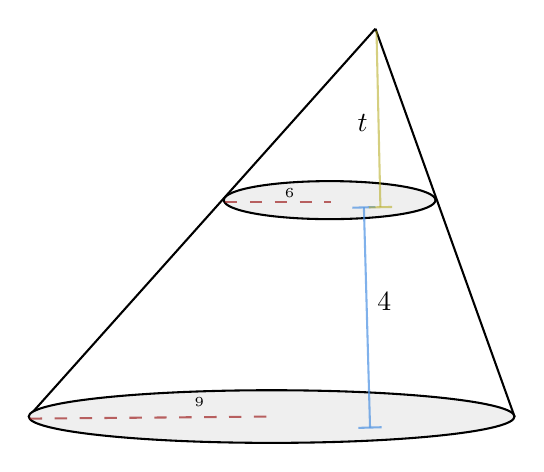
\begin{tikzpicture}[x=0.75pt,y=0.75pt,yscale=-1,xscale=1]
%uncomment if require: \path (0,701); %set diagram left start at 0, and has height of 701

%Straight Lines [id:da8181035772508525] 
\draw    (310.78,28.17) -- (143.72,215.03) ;
%Shape: Ellipse [id:dp46228756305368] 
\draw  [fill={rgb, 255:red, 239; green, 239; blue, 239 }  ,fill opacity=1 ] (143.72,215.03) .. controls (143.72,208.03) and (196.12,202.35) .. (260.75,202.35) .. controls (325.38,202.35) and (377.78,208.03) .. (377.78,215.03) .. controls (377.78,222.03) and (325.38,227.71) .. (260.75,227.71) .. controls (196.12,227.71) and (143.72,222.03) .. (143.72,215.03) -- cycle ;
%Straight Lines [id:da015371876231234483] 
\draw    (310.78,28.17) -- (377.78,215.03) ;
%Shape: Ellipse [id:dp5932760100545671] 
\draw  [fill={rgb, 255:red, 239; green, 239; blue, 239 }  ,fill opacity=1 ] (237.72,110.76) .. controls (237.72,105.7) and (260.55,101.6) .. (288.71,101.6) .. controls (316.87,101.6) and (339.69,105.7) .. (339.69,110.76) .. controls (339.69,115.82) and (316.87,119.92) .. (288.71,119.92) .. controls (260.55,119.92) and (237.72,115.82) .. (237.72,110.76) -- cycle ;
%Straight Lines [id:da6466751329195175] 
\draw [color={rgb, 255:red, 74; green, 144; blue, 226 }  ,draw opacity=0.7 ]   (305.21,114.26) -- (308.17,220.33) ;
\draw [shift={(308.17,220.33)}, rotate = 268.4] [color={rgb, 255:red, 74; green, 144; blue, 226 }  ,draw opacity=0.7 ][line width=0.75]    (0,5.59) -- (0,-5.59)   ;
\draw [shift={(305.21,114.26)}, rotate = 268.4] [color={rgb, 255:red, 74; green, 144; blue, 226 }  ,draw opacity=0.7 ][line width=0.75]    (0,5.59) -- (0,-5.59)   ;
%Straight Lines [id:da11484541699420614] 
\draw [color={rgb, 255:red, 156; green, 25; blue, 25 }  ,draw opacity=0.67 ] [dash pattern={on 4.5pt off 4.5pt}]  (238.22,111.76) -- (289.21,111.76) ;
%Straight Lines [id:da2635291794376522] 
\draw [color={rgb, 255:red, 156; green, 25; blue, 25 }  ,draw opacity=0.67 ] [dash pattern={on 4.5pt off 4.5pt}]  (144.22,216.03) -- (260.75,215.03) ;
%Straight Lines [id:da7830962643074002] 
\draw [color={rgb, 255:red, 181; green, 170; blue, 28 }  ,draw opacity=0.56 ]   (311.28,29.17) -- (313.17,114.17) ;
\draw [shift={(313.17,114.17)}, rotate = 268.73] [color={rgb, 255:red, 181; green, 170; blue, 28 }  ,draw opacity=0.56 ][line width=0.75]    (0,5.59) -- (0,-5.59)   ;


% Text Node
\draw (222.17,204.5) node [anchor=north west][inner sep=0.75pt]  [font=\tiny]  {$9$};
% Text Node
\draw (265.67,103.5) node [anchor=north west][inner sep=0.75pt]  [font=\tiny]  {$6$};
% Text Node
\draw (300.67,68) node [anchor=north west][inner sep=0.75pt]    {$t$};
% Text Node
\draw (310.17,154) node [anchor=north west][inner sep=0.75pt]    {$4\ \text{}$};


\end{tikzpicture}
\end{center}

Since the cone is not fully formed then we can extend the height to a point that makes the cone full. In this case, the extended line will be $t$. Next, since the smaller cone and the bigger cone are similar, then we can conclude that $$\dfrac{t}{6} = \dfrac{t+4}{9}$$. Finding $t$, we have $t=8.$

\newpage

Now, we completed the figure, we can find the volume of the bowl and that is the difference of the volume of the whole cone and the smaller cone. In mathematical terms, its:

$$V_{B} = V_L - V_S = \left(\pi(9)^2(t+4) \right) - \left(\pi(6)^2(t) \right) = \pi \left(81(12)  - 36(8)\right) = 684\pi.$$ Hence, the volume is \fbox{$684 \pi.$}

\begin{probboxed}[\href{http://pmo.ph/wp-content/uploads/2020/11/19th-PMO-Area-Stage-Questions-and-Answers.pdf}{PMO 19 Areas I.5}] 

In parallelogram $ABCD$, $AB=1, BC =4,$ and $\angle ABC = 60^{\circ}$. Suppose that $AC$ is extended from $A$ to a point $E$ beyond $C$ so that triangle $ADE$ has the same area as the parallelogram. Find the length of $DE.$

\end{probboxed}

\ans{$2\sqrt{3}$}

\sol

Refer to the figure below (figure not drawn to scale:)

\begin{center}



\tikzset{every picture/.style={line width=0.75pt}} %set default line width to 0.75pt        

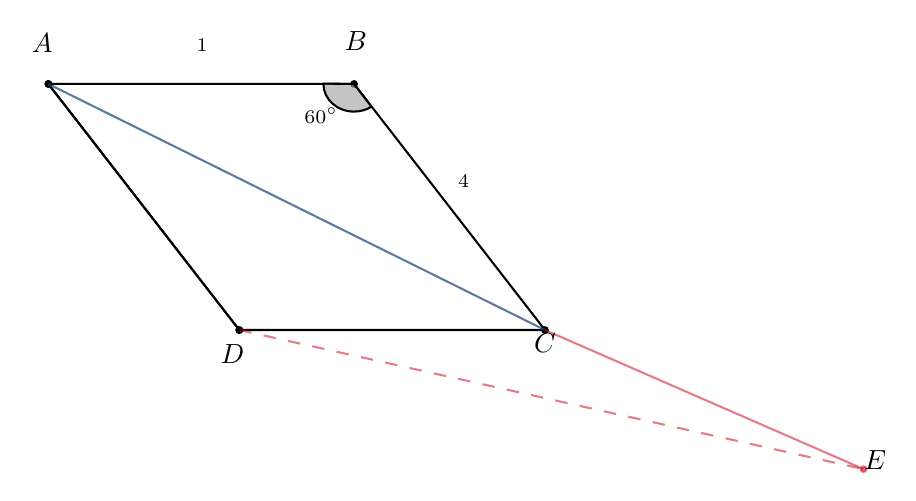
\begin{tikzpicture}[x=0.75pt,y=0.75pt,yscale=-1,xscale=1]
%uncomment if require: \path (0,1195); %set diagram left start at 0, and has height of 1195

%Shape: Rectangle [id:dp8592248193003178] 
\draw   (51.39,972.47) -- (198.68,972.47) -- (290.68,1091.03) -- (143.39,1091.03) -- cycle ;
%Straight Lines [id:da0960041213483327] 
\draw    (51.39,972.47) -- (143.39,1091.03) ;
\draw [shift={(143.39,1091.03)}, rotate = 52.19] [color={rgb, 255:red, 0; green, 0; blue, 0 }  ][fill={rgb, 255:red, 0; green, 0; blue, 0 }  ][line width=0.75]      (0, 0) circle [x radius= 1.34, y radius= 1.34]   ;
\draw [shift={(51.39,972.47)}, rotate = 52.19] [color={rgb, 255:red, 0; green, 0; blue, 0 }  ][fill={rgb, 255:red, 0; green, 0; blue, 0 }  ][line width=0.75]      (0, 0) circle [x radius= 1.34, y radius= 1.34]   ;
%Straight Lines [id:da19112836734025374] 
\draw    (51.39,972.47) -- (198.68,972.47) ;
\draw [shift={(198.68,972.47)}, rotate = 0] [color={rgb, 255:red, 0; green, 0; blue, 0 }  ][fill={rgb, 255:red, 0; green, 0; blue, 0 }  ][line width=0.75]      (0, 0) circle [x radius= 1.34, y radius= 1.34]   ;
\draw [shift={(51.39,972.47)}, rotate = 0] [color={rgb, 255:red, 0; green, 0; blue, 0 }  ][fill={rgb, 255:red, 0; green, 0; blue, 0 }  ][line width=0.75]      (0, 0) circle [x radius= 1.34, y radius= 1.34]   ;
%Straight Lines [id:da8421038388814408] 
\draw    (143.39,1091.03) -- (290.68,1091.03) ;
\draw [shift={(290.68,1091.03)}, rotate = 0] [color={rgb, 255:red, 0; green, 0; blue, 0 }  ][fill={rgb, 255:red, 0; green, 0; blue, 0 }  ][line width=0.75]      (0, 0) circle [x radius= 1.34, y radius= 1.34]   ;
\draw [shift={(143.39,1091.03)}, rotate = 0] [color={rgb, 255:red, 0; green, 0; blue, 0 }  ][fill={rgb, 255:red, 0; green, 0; blue, 0 }  ][line width=0.75]      (0, 0) circle [x radius= 1.34, y radius= 1.34]   ;
%Shape: Pie [id:dp7629928757272058] 
\draw  [fill={rgb, 255:red, 155; green, 155; blue, 155 }  ,fill opacity=0.58 ] (207.1,983.42) .. controls (204.71,984.91) and (201.81,985.79) .. (198.68,985.79) .. controls (190.53,985.79) and (183.92,979.83) .. (183.92,972.47) .. controls (183.92,972.41) and (183.92,972.36) .. (183.92,972.3) -- (198.68,972.47) -- cycle ;
%Straight Lines [id:da47047810848533245] 
\draw [color={rgb, 255:red, 25; green, 68; blue, 118 }  ,draw opacity=0.71 ]   (51.39,972.47) -- (290.68,1091.03) ;
%Straight Lines [id:da52655044101743] 
\draw [color={rgb, 255:red, 208; green, 2; blue, 27 }  ,draw opacity=0.52 ]   (290.68,1091.03) -- (444.13,1158.03) ;
%Straight Lines [id:da6572801279812626] 
\draw [color={rgb, 255:red, 208; green, 2; blue, 27 }  ,draw opacity=0.52 ] [dash pattern={on 4.5pt off 4.5pt}]  (143.39,1091.03) -- (444.13,1158.03) ;
\draw [shift={(444.13,1158.03)}, rotate = 12.56] [color={rgb, 255:red, 208; green, 2; blue, 27 }  ,draw opacity=0.52 ][fill={rgb, 255:red, 208; green, 2; blue, 27 }  ,fill opacity=0.52 ][line width=0.75]      (0, 0) circle [x radius= 1.34, y radius= 1.34]   ;


% Text Node
\draw (247.33,1014.7) node [anchor=north west][inner sep=0.75pt]  [font=\scriptsize]  {$4$};
% Text Node
\draw (121.33,949.36) node [anchor=north west][inner sep=0.75pt]  [font=\scriptsize]  {$1$};
% Text Node
\draw (442.95,1147.61) node [anchor=north west][inner sep=0.75pt]    {$E$};
% Text Node
\draw (173.27,982.54) node [anchor=north west][inner sep=0.75pt]  [font=\scriptsize]  {$60^{\circ }$};
% Text Node
\draw (283.93,1091.36) node [anchor=north west][inner sep=0.75pt]    {$C$};
% Text Node
\draw (132.93,1096.53) node [anchor=north west][inner sep=0.75pt]    {$D$};
% Text Node
\draw (192.6,945.87) node [anchor=north west][inner sep=0.75pt]    {$B$};
% Text Node
\draw (41.93,946.87) node [anchor=north west][inner sep=0.75pt]    {$A$};


\end{tikzpicture}
\end{center}

\vspace{-1em}

Finding the area of the parallelogram, that is, the twice the area of $\Delta ABC$, which the whole area of the parallelogram is equivalent to $2\sqrt{3}$. Draw an altitude from $D$ to line $AC.$ and denote it $h$ and let be the point of its foot be $Y.$

\begin{center}



\tikzset{every picture/.style={line width=0.75pt}} %set default line width to 0.75pt        

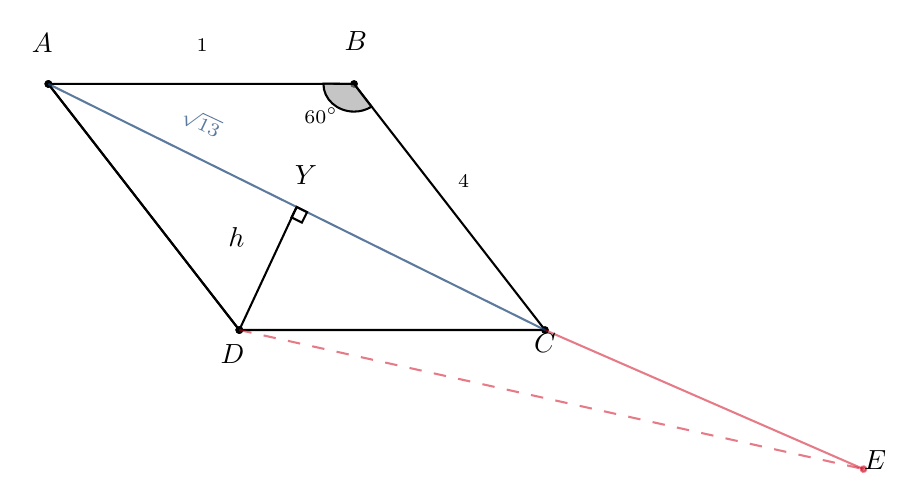
\begin{tikzpicture}[x=0.75pt,y=0.75pt,yscale=-1,xscale=1]
%uncomment if require: \path (0,1195); %set diagram left start at 0, and has height of 1195

%Shape: Rectangle [id:dp38960622976141934] 
\draw   (67.39,732.98) -- (214.68,732.98) -- (306.68,851.53) -- (159.39,851.53) -- cycle ;
%Straight Lines [id:da2890224948589972] 
\draw    (67.39,732.98) -- (159.39,851.53) ;
\draw [shift={(159.39,851.53)}, rotate = 52.19] [color={rgb, 255:red, 0; green, 0; blue, 0 }  ][fill={rgb, 255:red, 0; green, 0; blue, 0 }  ][line width=0.75]      (0, 0) circle [x radius= 1.34, y radius= 1.34]   ;
\draw [shift={(67.39,732.98)}, rotate = 52.19] [color={rgb, 255:red, 0; green, 0; blue, 0 }  ][fill={rgb, 255:red, 0; green, 0; blue, 0 }  ][line width=0.75]      (0, 0) circle [x radius= 1.34, y radius= 1.34]   ;
%Straight Lines [id:da5498902381038238] 
\draw    (67.39,732.98) -- (214.68,732.98) ;
\draw [shift={(214.68,732.98)}, rotate = 0] [color={rgb, 255:red, 0; green, 0; blue, 0 }  ][fill={rgb, 255:red, 0; green, 0; blue, 0 }  ][line width=0.75]      (0, 0) circle [x radius= 1.34, y radius= 1.34]   ;
\draw [shift={(67.39,732.98)}, rotate = 0] [color={rgb, 255:red, 0; green, 0; blue, 0 }  ][fill={rgb, 255:red, 0; green, 0; blue, 0 }  ][line width=0.75]      (0, 0) circle [x radius= 1.34, y radius= 1.34]   ;
%Straight Lines [id:da5501262293792855] 
\draw    (159.39,851.53) -- (306.68,851.53) ;
\draw [shift={(306.68,851.53)}, rotate = 0] [color={rgb, 255:red, 0; green, 0; blue, 0 }  ][fill={rgb, 255:red, 0; green, 0; blue, 0 }  ][line width=0.75]      (0, 0) circle [x radius= 1.34, y radius= 1.34]   ;
\draw [shift={(159.39,851.53)}, rotate = 0] [color={rgb, 255:red, 0; green, 0; blue, 0 }  ][fill={rgb, 255:red, 0; green, 0; blue, 0 }  ][line width=0.75]      (0, 0) circle [x radius= 1.34, y radius= 1.34]   ;
%Shape: Pie [id:dp028088096122260486] 
\draw  [fill={rgb, 255:red, 155; green, 155; blue, 155 }  ,fill opacity=0.58 ] (223.1,743.92) .. controls (220.71,745.42) and (217.81,746.3) .. (214.68,746.3) .. controls (206.53,746.3) and (199.92,740.33) .. (199.92,732.98) .. controls (199.92,732.92) and (199.92,732.86) .. (199.92,732.8) -- (214.68,732.98) -- cycle ;
%Straight Lines [id:da29670473936363995] 
\draw [color={rgb, 255:red, 25; green, 68; blue, 118 }  ,draw opacity=0.71 ]   (67.39,732.98) -- (306.68,851.53) ;
%Straight Lines [id:da5676473218871667] 
\draw [color={rgb, 255:red, 208; green, 2; blue, 27 }  ,draw opacity=0.52 ]   (306.68,851.53) -- (460.13,918.53) ;
%Straight Lines [id:da7782622713600449] 
\draw    (187.03,792.25) -- (159.39,851.53) ;
%Shape: Square [id:dp2577415814559363] 
\draw   (187.03,792.25) -- (192.05,794.75) -- (189.55,799.76) -- (184.54,797.27) -- cycle ;
%Straight Lines [id:da5242282156631957] 
\draw [color={rgb, 255:red, 208; green, 2; blue, 27 }  ,draw opacity=0.52 ] [dash pattern={on 4.5pt off 4.5pt}]  (159.39,851.53) -- (460.13,918.53) ;
\draw [shift={(460.13,918.53)}, rotate = 12.56] [color={rgb, 255:red, 208; green, 2; blue, 27 }  ,draw opacity=0.52 ][fill={rgb, 255:red, 208; green, 2; blue, 27 }  ,fill opacity=0.52 ][line width=0.75]      (0, 0) circle [x radius= 1.34, y radius= 1.34]   ;

% Text Node
\draw (153.11,800.29) node [anchor=north west][inner sep=0.75pt]  [rotate=-2.28]  {$h$};
% Text Node
\draw (57.93,707.37) node [anchor=north west][inner sep=0.75pt]    {$A$};
% Text Node
\draw (208.6,706.37) node [anchor=north west][inner sep=0.75pt]    {$B$};
% Text Node
\draw (148.93,857.04) node [anchor=north west][inner sep=0.75pt]    {$D$};
% Text Node
\draw (299.93,851.87) node [anchor=north west][inner sep=0.75pt]    {$C$};
% Text Node
\draw (189.27,743.04) node [anchor=north west][inner sep=0.75pt]  [font=\scriptsize]  {$60^{\circ }$};
% Text Node
\draw (458.95,908.12) node [anchor=north west][inner sep=0.75pt]    {$E$};
% Text Node
\draw (137.33,709.87) node [anchor=north west][inner sep=0.75pt]  [font=\scriptsize]  {$1$};
% Text Node
\draw (263.33,775.2) node [anchor=north west][inner sep=0.75pt]  [font=\scriptsize]  {$4$};
% Text Node
\draw (133.63,740.88) node [anchor=north west][inner sep=0.75pt]  [font=\scriptsize,color={rgb, 255:red, 25; green, 68; blue, 118 }  ,opacity=0.71 ,rotate=-25.15]  {$\sqrt{13}$};
% Text Node
\draw (184.67,770.6) node [anchor=north west][inner sep=0.75pt]    {$Y$};


\end{tikzpicture}
\end{center}

To find $h$, note that the area of $\Delta ADC$ is $\sqrt{3}$, and by the law of cosines, $AC = \sqrt{13}$ such that $$\dfrac{1}{2} \left(\sqrt{13} \right)h = \sqrt{3}$$ and we obtain $h = \dfrac{2\sqrt{39}}{13}$. Next, we will find $AY$ and by Pythagorean's theorem, $AY = \dfrac{14\sqrt{13}}{13}$. Now, we are steps closer to find $DE$. But we are not done yet. So, we are motivated to find the length of $AE$, and that is equivalent to $$\implies \dfrac{1}{2} \left(AE \right)h = 2\sqrt{3} \implies AE = \dfrac{4\sqrt{3}}{DY} \implies \dfrac{4\sqrt{3}}{\dfrac{2\sqrt{39}}{13}} = 4\sqrt{3} \cdot {\dfrac{13}{2\sqrt{39}}} = 2\sqrt{13}. $$ This implies that $CE = AC$. Next, subtract the length of $AY$ from $AE$ for us to find $YE$, and by subtraction, we have $$YE = 2\sqrt{13} -\dfrac{14\sqrt{13}}{13} = \dfrac{12\sqrt{13}}{13}$$

\vspace{2mm}


Now, we got the necessary information to find $DE$, we can invoke the Pythagorean theorem: $$DE = \sqrt{DY^2 + YE^2} = \sqrt{\left(\dfrac{2\sqrt{39}}{13}\right)^2 + \left(\dfrac{12\sqrt{13}}{13}\right)^2} = \sqrt{\dfrac{156}{13}} = 2\sqrt{3}$$. Hence, the value of $DE$ is \fbox{$2\sqrt{3}.$}

\begin{probboxed}[\href{https://pmo.ph/wp-content/uploads/2019/01/21st-PMO-Area-Stage.pdf}{PMO 21 Areas I.20}]
Suppose that $a, b, c$ are real numbers such that

$$\dfrac{1}{a} + \dfrac{1}{b} + \dfrac{1}{c} = 4\left( \dfrac{1}{a+b} + \dfrac{1}{b+c} + \dfrac{1}{c+a} \right) = \dfrac{c}{a+b} + \dfrac{a}{b+c} + \dfrac{b}{c+a} = 4$$.

Determine the value of $abc.$


\end{probboxed}

\ans{$\dfrac{49}{23}$}

\sol

Let $abc = k$. To solve this problem, our goal is to determine a polynomial with the roots of $a,b$ and $c$ such that $$x^3 - (a+b+c)x^2 + (ab+bc+ca)x -abc = 0$$ $\forall a,b,c \in \mathbb{R}$. Denote the polynomial as $P(x)$.

\vspace{2mm}

First, we need to find $a+b+c$:

\begin{center}
    \begin{equation*}
        \begin{array}{llll}
             \implies & (a+b+c)\left( \dfrac{1}{a+b} + \dfrac{1}{b+c} + \dfrac{1}{c+a} \right) & = & 3 + \dfrac{c}{a+b} + \dfrac{a}{b+c} + \dfrac{b}{c+a} \\
             
             \\
             
             \implies & \hspace{46mm} (a+b+c) & = & 7 \\                         
        \end{array}
    \end{equation*}
\end{center}

Next, we suppose to find $ab+bc+ca$ because we know that $$
\dfrac{1}{a} + \dfrac{1}{b} + \dfrac{1}{c} = \dfrac{ab+bc+ca}{abc}=4$$. But with the given information, we have, it would become tedious. However, notice that $\dfrac{1}{a+b} + \dfrac{1}{b+c} + \dfrac{1}{c+a}$ can be rewritten as $$\dfrac{1}{7-a} + \dfrac{1}{7-b} + \dfrac{1}{7-c} = 1$$. If we write this in this way, this is actually the sum of the reciprocals of the roots of the polynomial $P(7-x)$. Rewritting the polynomial as $P(7-x)$, we have:

\vspace{-2em}

\begin{center}
    \begin{equation*}
        \begin{array}{lll}
             \implies P(7-x) & = & (7-x)^3 - 7(7-x)^2 + 4k(7-x) - k = 0  \\
             
             \\
             
             \implies P(7-x) & = & (343 + 147x -21x^2 - x^3) - (343 - 98x + 7x^2)  + (28k - 4kx) - k = 0  \\
             
             \\
             
             \implies P(7-x) & = & −x^3 + 14x^2 - (49 + 4k)x + 27k = 0\\
        \end{array}
    \end{equation*}
\end{center}

Now, we have a sufficient information, we conclude that $$\dfrac{- (49 + 4k)}{-27k} = 1 \implies 49 + 4k = 27k \implies abc = \dfrac{49}{23}.$$

Hence, we got the final answer

\begin{probboxed}[\href{https://www.facebook.com/cediesmathverse/posts/478611540322117}{Cedie's Mathverse Problem 3B}]

Find, with proof, all nonnegative integer triples $(x,y,z)$ such that $3^x = 7^y + 2^z$.


\end{probboxed}

\ans{$(2,1,1), (1,0,1), (2,0,3), (4,2,5)$}

\sol

By observation, we see that $(2,1,1)$ and $(1,0,1)$ are solutions. Now, we got these solutions, does it mean these are only solutions? Well, this is where the proof comes in.

\vspace{2mm}

By modulo 2, we have $(1)^x = (-1)^y$ or $(-1)^x = 1^y$, and we will name them Case 1 and Case 2, respectively. For Case 1, notice that $x$ can be odd or even while $y$ must be even. For Case 2, it is the vice versa of Case 1. In this case, we obtain a solution, which is $(4,2,5)$.

\vspace{2mm}

By modulo 3, we have $0 \equiv 1^y + (-1)^z$. Notice that $y$ can be any number while $z$ must be odd or in other words, $z=2k+1$ for some non-negative integer $k$. Using this case, we should obtain $(2,0,3)$.

\vspace{2mm}

Hence, our solutions are \fbox{$(2,1,1), (1,0,1), (2,0,3), (4,2,5)$} and we are done!



\section*{Closing remarks}
Thank you for reading this write-up. There will be a \joshbf{PART II} of this and it will be released this Friday or Saturday. As always, if you see any typos, and if you have clarifications, you can contact me at \mailto{jrdobaob@addu.edu.ph }.


\vspace{87mm}

\begin{center}

\includegraphics[width=3.5in]{JOSH ROBERT OBAOB (2).png}
\end{center}



\end{document}
